%  Prerequisites
\chapter{State of the Art}
This chapter provides an overview of the concepts and technologies that are necessary for our current work. First, we define domain-specific terms in section \ref{lab:background}. We describe the technologies used in the implementation in section \ref{lab:systems}.

\section{Background} \label{lab:background}

This section introduces the concepts, which are relevant to the implementation part of this thesis.

\subsection{Social Bots and Chatbots}\label{sec:chatbots}
Bots are interfaces, providing automated services to end-users.
In contrast to traditional computer programs, bots can use the same services and perform the same actions as human users. Those actions include browsing web pages or issuing API calls.
\begin{quote}
    ``A social bot is a computer algorithm that automatically produces content and interacts with humans on social media, [...]'' \cite{FVD*16b}
\end{quote}
Social bots are interacting with users in human-like conversations.
Social bots are getting more and more popular in Human-Computer Interaction (HCI), as they integrate automation into the daily lives of people \cite{BFPN17}. Users interact with a social bot through a dedicated channel like the chat functionality of a social network.
Social bots, which use chat platforms, are called chatbots, or conversational bots \cite{WWX*16,AAA17}.
Chatbots have recently become very popular in the context of customer care \cite{CHW*17,FVD*16b}, where they act as virtual assistants, which can answer simple questions \cite{CaWh14} or perform predefined tasks. 
Their simplicity allows even non-experienced users to perform actions of various degrees of difficulty. 
Chatbots can assist companies in customer service, allowing staff to concentrate on less mundane issues with customers. This increases the effectiveness of the service while lowering costs. \cite{AAA17}

% Chatbots can be classified into chit-chat chatbots, or task-oriented bots.
% A chit-chat bot engages users into interesting conversations and focusses more on the actual conversation. Task-oriented bots are focused on getting certain actions done. As soon as the desired action is done, the bot will stop the conversation. 

We can distinguish between retrieval-based chatbots and generic chatbots \cite{NLKl19,WWX*16}.
Retrieval-based bots are more focused on getting specific tasks done than engaging in a coherent conversation.
Retrieval-based chatbots measure the similarity of user queries to candidate responses and run the task that is defined for that response.

Generic chatbots, on the other hand, also produce generic responses.
An advantage of generic chatbots is that they provide a better user experience as users can interact more naturally with them than with retrieval-based chatbots.

Chatbots use natural language processing techniques to determine what the user wants to do.
Chatbots provide a better user experience \cite{CHW*17} than traditional command-based tools because the user is not required to memorize commands to get the desired results.
Thus, even non-trained users can use such chatbots.
Users can interact with them in a familiar environment. 
Therefore, chatbots are desirable as assistants.

\subsubsection{Natural Language Understanding}\label{sec:NLU}
Natural Language Understanding (NLU) is a branch of Artificial Intelligence (AI), which aims to make computer programs understand human language.
NLU transforms a block of input text into a data structure that is programmer-friendly but still describes the original meaning of the text \cite{CWB*11}.

Most actual NLU algorithms look only at the syntax of words, which relies on statistical features, such as word occurrence frequency \cite{CaWh14}.
However, humans consider far more information. The reading of a word triggers related concepts and experiences. Those experiences are combined to deduce the meaning of a text.

Computers try to close this knowledge gap with computational models, which emulate human cognitive processing.
By evaluating the results of those models for a given input, researchers can incrementally improve the accuracy of the model. \cite{CaWh14}
NLU is a domain that is a key research topic for companies like Google and Facebook. \cite{AAA17}


\subsection{Communities of Practice}\label{sec:CoP}
A Community of Practice (CoP) is a special kind of community consisting of members studying a particular domain.
\begin{quote}
    ``
    Communities of practice are groups of people who share a concern or a passion for something they do and learn how to do it better as they interact regularly.''  \cite{Weng98}
\end{quote}
In contrast to traditional knowledge systems, where a student passively receives his information, the learner is actively participating in the community by voluntarily sharing his knowledge with other members of the community \cite{AMMi15,Kern08}.
The advantage of CoPs is that they make the learning process easier \cite{SaAr05} and the transfer of knowledge faster \cite{CuZe05}.

Members of a CoP have different degrees of knowledge of the domain.
For example, a student has less knowledge than a researcher in a specific domain.
Furthermore, members have various degrees of interest in the practice of the community.
Members with a lot of interest in that domain tend to know more about it and tend to contribute more to the community.
Such members are called \emph{core members} of the community.
Members, which are less active in the community are called \emph{lurkers}.

Members of CoPs do not have to belong to the same organization but participate in common work through social interactions \cite{Weng98}. In the case of an online CoP, this could be an online social network \cite{CuZe05}. Multiple, overlapping, CoPs can communities can exist inside a single CoP.

\subsection{Measurement of Success}
Communities need to constantly be aware of their successes and failures to improve their work and adjust to current requirements.
A general model for success does not exist, as communities are very diverse, dynamic, and informal structures with permeable boundaries.
The members of the community thus can be active participators in the community success modeling, as the success factors are relevant to the practice of the community members \cite{RKJa15}.

The community must continuously adjust the success factors of the success model to satisfy current requirements. Success factors can be internal aspects, like project duration, cost, and quality. Success factors can also be external aspects, like customer satisfaction \cite{AgRa06}.

It is important to note that a project can be evaluated from different perspectives \cite{RKJa15}, like the developers, the customers, or the end-users.
In each of these perspectives, each dimension of success can be more or less valuable.
DeLone and McLean \cite{DeMc92} base their model on six different interdependent measures:
\begin{itemize}
    \item \textbf{System Quality} are factors that describe the technical specifications of the system, such as service response time and scalability.
    \item \textbf{Information Quality} are factors about content quality, such as understandability and conciseness.
    \item \textbf{Use} are factors about how a system is used, such as the regularity of use by individual users or for the whole community.
    \item \textbf{User Satisfaction} includes factors describing users' personal experiences and is thereby largely subjective.
    \item \textbf{Individual Impact} are factors about how a user adapts to the system over time, such as task performance.
    \item \textbf{Organizational (or Community) Impact} includes factors about how the system influences the organization (or community) over time.
\end{itemize}
\begin{figure}[!h]
    \centering
    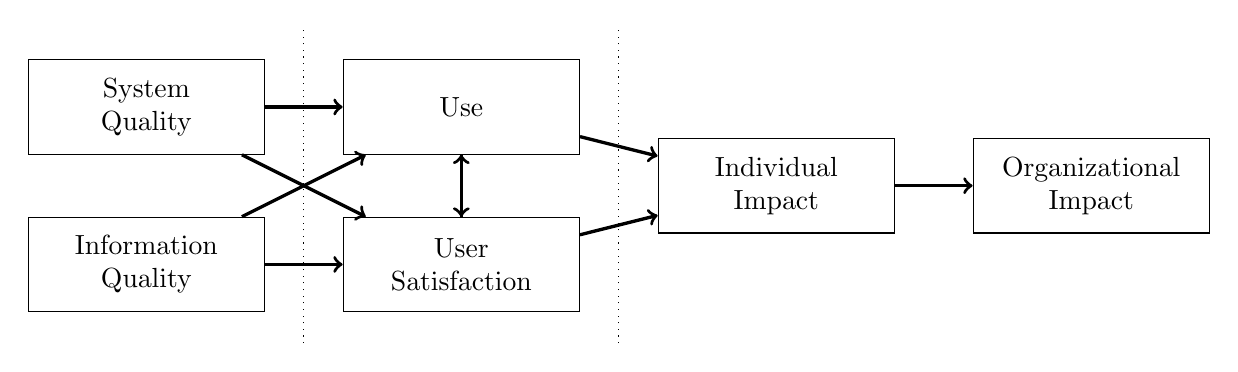
\begin{tikzpicture}[node distance=3.0cm and 6.0cm]
        \node[draw, align=center, minimum width=3cm, minimum height=1.2cm] at (0,2) (SysQ) {System\\ Quality};
        \node[draw, align=center, minimum width=3cm, minimum height=1.2cm] at (0,0) (InfoQ) {Information\\ Quality};
        \node[draw, align=center, minimum width=3cm, minimum height=1.2cm] at (4,2) (Use) {Use};
        \node[draw, align=center, minimum width=3cm, minimum height=1.2cm] at (4,0) (UserSat) {User\\ Satisfaction};
        \node[draw, align=center, minimum width=3cm, minimum height=1.2cm] at (8,1) (Indivi) {Individual\\ Impact};
        \node[draw, align=center, minimum width=3cm, minimum height=1.2cm] at (12,1) (Orga) {Organizational\\ Impact};
        \draw [->, very thick] (InfoQ) -- (Use);
        \draw [->, very thick] (InfoQ) -- (UserSat);
        \draw [->, very thick] (SysQ) -- (Use);
        \draw [->, very thick] (SysQ) -- (UserSat);
        \draw [->, very thick] (Use) -- (Indivi);
        \draw [->, very thick] (UserSat) -- (Indivi);
        \draw [->, very thick] (Use) -- (UserSat);
        \draw [->, very thick] (UserSat) -- (Use);
        \draw [->, very thick] (Indivi) -- (Orga);
        \draw[dotted] (2,-1) -- (2,3);
        \draw[dotted] (6,-1) -- (6,3);
    \end{tikzpicture}
    \caption{Community Information Systems Success Model by DeLone and McLean~\cite{DeMc92}}
    \label{CISModel}
\end{figure}
In order to collect data for the metrics, one should follow the principle \cite{RKJa15}:
\begin{quotation}
    ``observe, where possible; only survey,	where inevitable.''
\end{quotation}

\subsection{MobSOS}
The Mobile Community Information System Oracle for Success (MobSOS) framework is a tool, which assists online communities in monitoring and evaluating services. The MobSOS success model extends the classical IS success model of DeLone and McLean (D\&M) by adding features, which were not covered by the original model, such as Quality of Service and mobility \cite{Renz08}.
The MobSOS Success Modelling concept is described as an iterative process. 

The MobSOS Continuous Community Analytics (CCA) services extend the MobSOS framework by providing visualizations of MobSOS data and the ability to add Mediabases \cite{Kers20}, which can be used for success visualizuations.

\subsection{Mediabase}
Storing Web 2.0 data is a challenging task due to the variety of different non-interoperable formats.
Mediabase is a concept that has been proposed to store Web 2.0 data in a dynamic way by delivering an analysis environment for Web Science data sets \cite{KlPe08}.
Mediabase uses graphs to model the generated data.
The nodes in those graphs are called \emph{Actors} and represent either a \emph{ Medium}, an \emph{Artifact}, a \emph{Member} or a \emph{Network}.
A \emph{ Medium} can be a blog or a wiki.
The \emph{Artifact} would be an individual entry.
The \emph{Network} represents the community in which the different \emph{Members} interact.
\emph{Members} do not have to be human but are assigned a specific role in the \emph{Network}.
\begin{figure}[h]
    \centering
    \includegraphics*[width=0.9\linewidth]{related_work/mediabase.png}
    \caption{Mediabase Overview \cite{Klam10e}}
\end{figure}
Furthermore, Mediabase includes \emph{Services}, like a \emph{Watcher} to inspect the data.
A Mediabase consists of a backend database, like DB2, or MySQL, crawler scripts, monitoring processes, and a frontend for visualization of data and user interaction.

This approach is favorable for the management of large scale-free dynamic social graphs.

\section{Systems} \label{lab:systems}
This section describes existing systems which will be used for the realization of this project.

\subsection{las2peer}
las2peer\footnotemark is a platform, which allows users to deploy their HTTP services with ease. 
It is a distributed platform based on peer-to-peer networks without a central authority \cite{KRdJ16}.
Each service is a \emph{node} in the network. Many nodes can form a peer-to-peer seed network, communicating through standard protocols. 
Data storage and communications are encrypted, adding an extra layer of security to las2peer services.
This allows even small communities to design and deploy secure las2peer services. 

New nodes can join the las2peer network by using the \emph{bootstrap} flag followed by the IP address of one of the nodes in the network. The service can be addressed by its \emph{ServiceAgent id}  or by listening to an arbitrary topic. It can address other services in the network in the same way. 

The services inside a network share a key-value store as a distributed hash table (DHT). The entries are stored on each node's host filesystem. The entries are encrypted by their author. Only the author can change the value of an entry.

\footnotetext{\href{https://las2peer.org/}{las2peer.org}}

Groups are a feature in las2peer for security and defining rights in a community. 
A user can create a group by generating a \emph{GroupAgent}. 

In order to communicate with the nodes of the las2peer network from outside, a \emph{WebConnector} can be started on a node. This connector handles REST requests to the services. A service can then be accessed over HTTP by the following URL scheme: 
\begin{lstlisting}
  http(s)://ip:port/serviceAlias/methodName
\end{lstlisting}
The \emph{serviceAlias} is a name, which identifies the service in the network. 

las2peer includes an editor for Modelling and Code Generation called Community Application Editor (CAE). 
The CAE follows a model-driven approach as the  las2peer services can be created by designing a model using the \emph{Canvas} widget. The editor can be used as a collaborative, near-real-time framework \cite{dND*16}. 

las2peer also includes a framework for community evaluation based on MobSOS. This framework can be used to monitor and evaluate the success data of community applications.

\subsubsection{MobSOS Data Processing}
The MobSOS Data Processing service collects logs from the Mensa service and the MobSOS Success Modelling service. 
Logging data in MobSOS can be done by using the listing \ref{lst:logging}
\begin{lstlisting}[caption=Example use of a MonitoringEvent,captionpos=b,label={lst:logging}]
    Context.get().monitorEvent(
        MonitoringEvent.SERVICE_CUSTOM_MESSAGE_X, data
    );
\end{lstlisting}.
The MonitoringEvent \texttt{enum} provides different events which are logged in the network. An overview of the different monitoring events can be found on GitHub \footnote{\href{https://github.com/rwth-acis/mobsos-data-processing/wiki/Built-In-Monitoring-Events}{GitHub: MonitoringEvent}}. 
Each service can use its own events by using the \texttt{MonitoringEvent.CUSTOM\_MESSAGE\_X}, where \emph{X} is a number between 1 and 99. 
Those \texttt{data} variables contains generic JSON data. This data provides information about how community members are using the service.
To monitor messages in the service, the service needs to be started using the \texttt{--observer} flag.
The data is stored in the MobSOS MySQL database under the \texttt{MESSAGE} table. The table contains a column \texttt{REMARKS} which is used to store the JSON data.

The MobSOS Data Processing service\footnotemark processes data, which are monitored in the context of a service in the network, and stores it in a database.

\footnotetext{\href{https://github.com/rwth-acis/mobsos-data-processing}{GitHub: Data Processing}}


\subsubsection{MobSOS Success Modelling}

The MobSOS Success Modelling service\footnotemark can be used in order to create and manage success models that follow the six success dimensions proposed by DeLone and McLean \cite{DeMc92}.
\footnotetext{\href{https://github.com/rwth-acis/mobsos-success-modeling}{GitHub: Success Modelling}}
Each group in a las2peer network can create multiple success models for each las2peer service in the network. 
The groups reflect the las2peer \emph{GroupAgent} and the services reflect the \emph{ServiceAgents} in the las2peer network.
The success model contains the six MobSOS dimensions.
\begin{lstlisting}[ caption=Example of a success model,language=XML ]
<SuccessModel name="Name of success model" 
    service="your.service.name@version">
    <dimension name="name of dimension 1">
        <factor name="Name of factor">
            <measure name="No Factors or Measures yet"/>
        </factor>
    </dimension>
    .
    .
    .
    <dimension name="name of dimension n">
        <factor name="Name of factor">
            <measure name="No Factors or Measures yet"/>
        </factor>
    </dimension>
</SuccessModel>
\end{lstlisting}
Each of these dimensions includes a list of success factors describing the dimension.
Each factor contains a list of success measures. The success measures are stored in a separate file called \emph{Measurement Catalog}. A measure defines how to get data and how to visualize it. 

Three types of visualization are supported
\begin{itemize}
    \item Value: This visualization returns a single value with an optional unit
    \item Chart: This visualization returns a chart as a picture. Different chart types from the Google Charts API\footnotemark are available.
    \item KPI: This visualization uses an arbitrary amount of queries, with each query returning a value. The values from the query can be combined through various mathematical operations.
\end{itemize}
\footnotetext{\href{https://developers.google.com/chart}{Google Charts}}


\subsection{Social Bot Framework}
The Social Bot Framework (SBF) is a Web-based model-driven near-real-time environment to develop chatbots \cite{NLKl19}. 
The model-driven development allows less experienced users to take part in the development process. This type of development is favorable for creating a chatbot inside a Community of Practice (CoP). 
The framework consists of a GUI and a Social Bot Manager Service.
The GUI of the Social Bot Framework (SBF) is used to model the bot and define the actions, which the bot should perform. 
The modeling space of the SBF can be used collaboratively. The modeling canvas is used to model the bot. Icons, representing elements of the bot, can be selected from the palette widget and connected with each other. 

The GUI also includes an NLU Model Training helper, which can be used to write training data for intent recognition using a Rasa server.
The resulting model is sent to the Social Bot Manager which deploys the bot and handles the communication with chat platforms, like \emph{Slack} \footnote{\href{https://slack.com/}{Slack}} or \emph{rocket.chat}\footnote{\href{https://rocket.chat/}{rocket.chat}}. 
The Social Bot Manager service\footnotemark is a las2peer service and can thereby call other las2peer services in the network. 
Thereby the bot can perform service requests to any service in a las2peer network.
\footnotetext{\href{https://github.com/rwth-acis/las2peer-social-bot-manager-service}{GitHub: Social Bot Manager}}

\subsection{RASA}
Rasa is an open-sourced framework for building chat- and voice-based bots. The goal of RASA is to bring current advances in machine-learning to end-users, such that they can create chatbots in a simple way \cite{BFPN17}. 
RASA is split into a component for natural-language understanding (RASA NLU), and a dialogue management component (RASA Core).

RASA NLU is used to extract the \emph{intents} and intent \emph{entities} of a user message.
The \emph{intent}\footnotemark of a message represents the thing that the user tries to accomplish. 
Entities are keywords that are relevant to the current context.
Intent recognition is done by using a text classification based on the fastText approach \cite{BFPN17}. 
fastText has similar accuracy to conventional deep learning classifiers but is much faster and more easily scalable \cite{JGBM16}.
\footnotetext{\href{https://rasa.com/docs/rasa/glossary\#intent}{Rasa: intents}}

RASA Core consists of a \emph{Tracker}, a \emph{Policy} and a set of \emph{Actions} \cite{BFPN17}. The Tracker manages the current state of the conversation. It gets an intent as input and forwards it the Policy, which selects the next Action, given the current state of the conversation and a predefined list of actions for each intent. The Action triggers the Tracker to recalculate the new state and might also send a reply to the user.

The system is built in a modularized way, with each service providing HTTP APIs \cite{BFPN17}. Thereby, the NLU component can be used independently of the rest of the framework, making it easy to integrate it into an existing system \cite{RaKe19}.


\subsection{Google Charts API}
Google Charts API\footnotemark is an API that provides visualizations for database data. The data, which should be visualized needs to be wrapped inside a JavaScript class called \texttt{DataTable}, which represents a two-dimensional table with rows and columns, where each column has a datatype.
A new column can be added using the \texttt{DataTable.addColumn} function, which takes the type and name as input. An example can be seen in Listing \ref{lst:gglCharts} from the Google Charts API documentation\footnotemark[\value{footnote}].

\begin{lstlisting}[caption=Example use of the DataTable class,captionpos=b,label={lst:gglCharts}]
var data = new google.visualization.DataTable();
data.addColumn('string', 'Topping');
data.addColumn('number', 'Slices');
data.addRows([
	['Mushrooms', 3],
	['Onions', 1],
	['Olives', 1], 
	['Zucchini', 1],
	['Pepperoni', 2]
]);
\end{lstlisting}
\footnotetext{\href{https://developers.google.com/chart}{Google Charts API}}

The visualizations are rendered as SVGs in the browser or downloaded as a PNG file by making a \texttt{http} call with the \texttt{getImageURI} as image URI parameter. 

\subsection{GraphQL}
GraphQL\footnotemark is a query language specification for web APIs.
\footnotetext{GraphQL: \href{https://graphql.github.io/}{https://graphql.github.io/}}
Instead of calling multiple endpoints for different requests, users can get all data from one endpoint by specifying what they need in a query. This prevents over- and under-fetching of data\footnotemark, thus increasing overall performance. This leads to a better user experience \cite{KKK20}.

\footnotetext{\href{https://www.howtographql.com/basics/1-graphql-is-the-better-rest}{https://www.howtographql.com/basics/1-graphql-is-the-better-rest}}

GraphQL does not mandate the use of a specific programming language, the actual implementation is up to the developer of the server. \footnotemark
\footnotetext{\href{http://spec.graphql.org/June2018/}{http://spec.graphql.org/June2018/}}
Many different implementations have been written for programming languages like Java \footnote{Java GraphQL Library:\href{https://www.graphql-java.com/documentation/master/}{https://www.graphql-java.com/documentation/master/}} and JavaScript. \footnote{JavaScript GraphQL Library:\href{https://www.npmjs.com/package/express-graphql}{https://www.npmjs.com/package/express-graphql}}

Transforming an existing REST API into a GraphQL API can be a cumbersome task \cite{WCL18}. That is why automation processes in the form of Wrappers have been proposed \cite{KKK20}, which convert an existing schema such as a Swagger schema into a GraphQL schema\footnote{\href{https://github.com/yarax/swagger-to-graphql}{Swagger-to-GraphQL}} \footnote{\href{https://github.com/IBM/openapi-to-graphql}{IBM: openapi-to-graphql}} \footnote{\href{https://github.com/rwth-acis/openapi-link-generator}{GitHub: Openapi Link Generator}}.   Such wrappers transform GraphQL requests into RESTful requests as depicted in Figure \ref{fig:graphqlWrapper}.
\begin{figure}
    \centering
    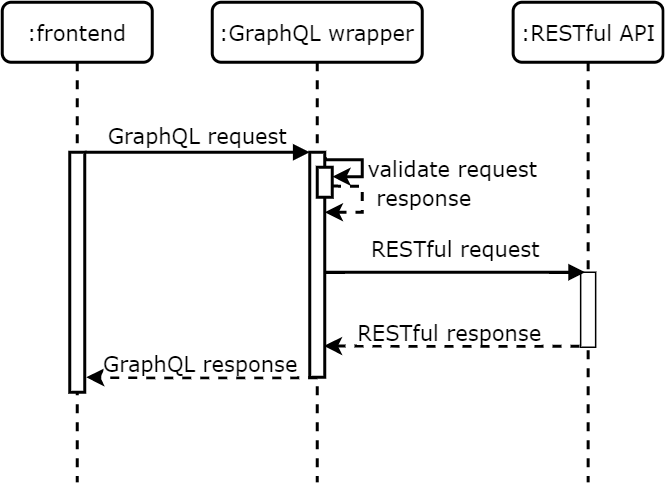
\includegraphics[width=0.6\linewidth]{realization/graphqlWrapper.png}
    \caption{Example of a GraphQL request}
    \label{fig:graphqlWrapper}
\end{figure}

In GraphQL, data objects are defined as a \emph{type}. GraphQL provides simple base-types like Int Float, Boolean, and String, but new types can also be defined. An example can be seen in \ref{lst:GraphQLType}. \\
\begin{lstlisting}[caption={Example of a GraphQL schema},captionpos=b,label={lst:GraphQLType}]
  type REVIEW { 
    dishId: String 
    mensaId: String 
    timestamp: String 
    stars: Int 
    comment:String
    author: String 
    id: ID 
  }
\end{lstlisting}
New fields can be dynamically added without influencing existing queries. The schemas are formalized as either a \emph{Query} or a \emph{Mutation}. They are declared by the keyword \emph{schema}. The query keyword can be omitted. An example of a query can be seen in listing \ref{lst:GraphQLQuery}.
\begin{lstlisting}[caption={Example of a GraphQL Query},captionpos=b,label={lst:GraphQLQuery}]
{
  REVIEW(id: "1000") {
    stars,
    author
  }
}
\end{lstlisting}
Here we access the rating of the review with the ID 1000.

Mutations are used to modify data. An example of a query can be seen in listing \ref{lst:GraphQLMut}.
\begin{lstlisting}[caption={Example of a GraphQL Mutation},captionpos=b,label={lst:GraphQLMut}]
mutation addReview(){
  {
  author
	stars 
  }
}
\end{lstlisting}

\subsection{Docker and Kubernetes}
Docker\footnotemark is an open-source containerizing technology, which aims to simplify and accelerate the development of web services.
\footnotetext{\href{https://www.docker.com/}{Docker}}
A Docker \emph{container} is a standalone executable package that contains all dependencies for the actual application. Docker containers run using the Docker \emph{engine}. Docker \emph{images} define the way a container should run, while the container is the actual runtime.
In contrast to virtual machines (VMs), Docker containers are virtualizations of the application layer instead of the physical hardware layer. Thereby, they take up less space (only a few MBs) and are faster to boot.
Docker images can be uploaded to Docker registries\footnotemark, which are central repositories for Docker images. 
\footnotetext{\href{https://docs.docker.com/docker-hub/}{Docker: Docker-hub}}

Kubernetes\footnotemark (K8s) is an open-source container orchestration tool, which automates deployment and scaling of a containerized application, like Docker containers. 
\footnotetext{\href{https://kubernetes.io/}{Kubernetes}}
K8s introduces an abstraction layer to containers called \emph{pods}. Pods can contain multiple containers. Pods are created and managed automatically by K8s. K8s also introduces \emph{services}, which serve as the communication endpoint of the pod, as it maps a single IP address to a pod. This is necessary as the IP address of the pod can change if it is restarted.
The different applications can communicate with each other using \texttt{http}. 
Different services and pods can be grouped together in \emph{name-spaces}.
K8s also has a service for DNS resolution. Each service gets its own domain in the form \texttt{my-service.my-namespace}.
